\documentclass[t, aspectratio=169]{beamer}
\usepackage{amsmath,amsfonts,amsthm,amstext,amssymb, xcolor, tikz, pgf, mathrsfs, polynom, pifont, tabto}

% ----------------------------------------------------------
% Theme Setup

% Use Metropolis Theme
\usetheme[numbering=fraction]{metropolis}
\setbeamertemplate{blocks}[rounded][shadow=false]
\makeatletter
\setlength{\metropolis@titleseparator@linewidth}{1pt}
\makeatother

% Define Colors
\definecolor{chargerblue}{HTML}{002764}
\definecolor{chargerred}{HTML}{e02034}
\definecolor{bggray}{HTML}{d0d3d4}

% Set Colors
\setbeamercolor{title}{fg=chargerblue}
\setbeamercolor{background canvas}{bg=white}
\setbeamercolor{title separator}{fg=chargerred}
\setbeamercolor{structure}{fg=chargerblue}
\setbeamercolor{frametitle}{fg=white, bg=chargerblue}
\setbeamercolor*{normal text}{fg=chargerblue}
\setbeamercolor*{block body}{bg=bggray}
\setbeamercolor*{block title}{bg=chargerblue, fg=white}
% ----------------------------------------------------------

% ----------------------------------------------------------
% Custom Definitions, Commands, Environments, etc.

% Sets of numbers
\def\R{\mathbb{R}} % The reals
\def\N{\mathbb{N}} % The naturals
\def\Z{\mathbb{Z}} % The integers
\def\Q{\mathbb{Q}} % The rationals

% Blank space
\newcommand{\blank}[1]{\underline{\hspace{#1}}} % Blank space

% Change font colors
\newcommand{\cyan}[1]{{\color{cyan}{#1}}} % Changes font to cyan
\newcommand{\red}[1]{{\color{red}{#1}}} % Changes font to red
\newcommand{\magenta}[1]{{\color{magenta}{#1}}} % Changes font to magenta
\newcommand{\orange}[1]{{\color{orange}{#1}}} % Changes font to orange
\newcommand{\yellow}[1]{{\color{yellow}{#1}}} % Changes font to yellow
\newcommand{\violet}[1]{{\color{violet}{#1}}} % Changes font to violet
\newcommand{\green}[1]{{\color{green}{#1}}} % Changes font to green
\newcommand{\blue}[1]{{\color{blue}{#1}}} % Changes font to blue
\newcommand{\white}[1]{{\color{white}{#1}}} % Changes font to white

% Fitted inclusion symbols
\newcommand{\fp}[1]{\left({#1}\right)} % Fitted parentheses around content
\newcommand{\fb}[1]{\left[{#1}\right]} % Fitted brackets
\newcommand{\lhoi}[1]{\left({#1}\right]} % Left half-open interval
\newcommand{\rhoi}[1]{\left[{#1}\right)} % Right half-open interval
\newcommand{\set}[1]{\left\{{#1}\right\}} % Fitted braces (useful for sets)
\newcommand{\av}[1]{\left|{#1}\right|} % Fitted absolute value bars

% Augmented Matrix Environment
\newenvironment{amatrix}[1]{%
	\left[\begin{array}{@{}*{#1}{c}|c@{}}
	}{%
	\end{array}\right]
}

% Miscellaneous
\def\then{\Rightarrow}
\def\to{\rightarrow}
\def\d{^{\circ}}
\newcommand{\?}{\stackrel{?}{=}}
\newcommand{\cmark}{\text{ \ding{51}}}
\newcommand{\xmark}{\text{ \ding{55}}}

% Coordinate Plane (Four-Quadrant)
\def\coordplane {
	\begin{tikzpicture}        \draw[step=0.25cm,black,very thin,opacity=0.25] (-2.5cm, -2.5cm) grid (2.5cm, 2.5cm);
		\draw[<->,thick,black] (-2.5cm, 0) -- (2.5cm, 0) node[anchor=north west,pos=0.94,font=\scriptsize]{$x$};
		\draw[<->,thick,black] (0,-2.5cm) -- (0, 2.5cm) node[anchor=south east,font=\scriptsize,pos=0.94]{$y$};
	\end{tikzpicture}
}

% Coordinate Plane (One-Quadrant)
\def\onequad {
	\begin{tikzpicture}
		\draw[step=0.25cm, black, very thin, opacity=0.25] (0,0) grid (7.5cm,5cm);
		\draw[->, thick, black] (0,0) -- (7.5cm, 0) node[anchor=north west,font=\scriptsize,pos=0.94]{$x$};
		\draw[->, black, thick] (0,0) -- (0,5cm) node[anchor=south east,font=\scriptsize,pos=0.94]{$y$};
	\end{tikzpicture}
}
% ----------------------------------------------------------

% ----------------------------------------------------------
% Presentation Information
\title[6-1]{Normal Distributions}
\subtitle{Section 6-1}
\author{Jacob Ayers}
\institute{Lesson \#17}
\date{MAT 110}
% ----------------------------------------------------------

\begin{document}
	
	% Slide 1 (Title Slide)
	\begin{frame}
		\titlepage
	\end{frame}
	
	% Slide 2 (Objectives)
	\begin{frame}{Objectives}
		\begin{itemize}
			\item Understand basic properties of normal distributions
			\item Find the area under the standard normal distribution, given various $z$ values
			\item Find a $z$ value, given an area under the standard curve.
		\end{itemize}
	\end{frame}

	\begin{frame}{Properties of Normal Distributions}
		The graph of a \textit{normal distribution} is continuous, bell-shaped, and symmetric.
		
		To illustrate each of these characteristics, here's a picture of the graph of a normally-distributed variable: \pause
		
		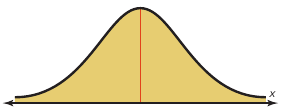
\includegraphics[width=3in]{norm-dist.png}
	\end{frame}

	\begin{frame}{Properties of Normal Distributions}
		The mean and standard deviation of a normal distribution affect its size and position. \pause \begin{itemize}
			\item Change in standard deviation = horizontal shrink or stretch
			\item Change in mean = horizontal translation
		\end{itemize}
	
		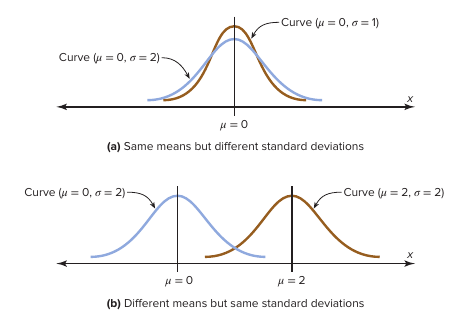
\includegraphics[width=3in]{norm-dist-adjust.png}
	\end{frame}

	\begin{frame}{Properties of Normal Distributions}
		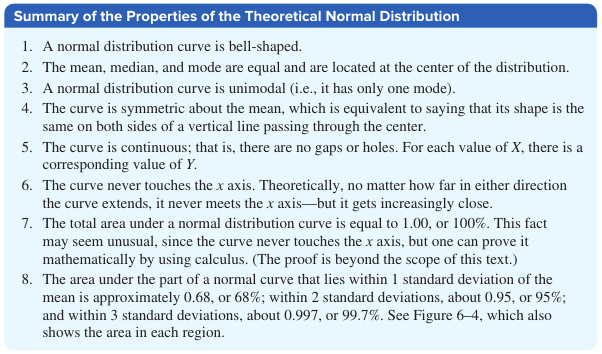
\includegraphics[width=5in]{norm-dist-prop.png}
	\end{frame}

	\begin{frame}{Properties of Normal Distributions}
		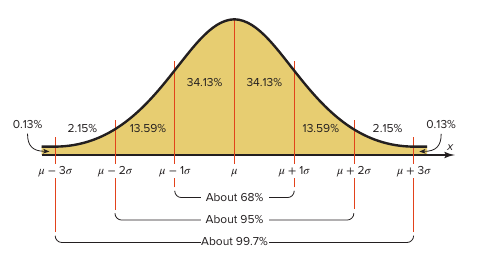
\includegraphics[width=4in]{norm-dist-percentages.png}
	\end{frame}

	\begin{frame}{The Standard Normal Distribution}
		The \textit{standard normal distribution} is a normal distribution whose mean is $0$ and whose standard deviation is $1$. \pause
		
		We use the standard normal distribution for convenience in calculations. \pause
		
		The primary calculation we are interested in doing is finding the area under the curve in a given region. \pause
		
		Table E in Appendix A (posted on Moodle) is a table listing areas under the curve at various $z$-scores (recall: $z = \dfrac{X - \mu}{\sigma}$) \pause
		
		We can also use a graphing calculator to do the calculations, but we'll learn to do that later.
	\end{frame}

	\begin{frame}{Areas Under the Standard Normal Distribution}
		Before we can start finding areas, we need to know how to use the table to look up areas associated with a given $z$-score. \pause
		
		Note that the values in the table correspond to the area to the \textit{left} of that $z$-score. \pause
		
		Example: in the table $z = 1.34$ maps to an area of $0.9099$. This means that the area to the left of $z = 1.34$ is $0.9099$. \pause
		
		Look up the area associated with each of the following $z$-scores:
		
		a) $z = -0.29$ \pause $0.3859$ \pause \\
		b) $z = 3.14$ \pause $0.9991$ \pause \\
		c) $z = 2.57$ \pause $0.9949$
	\end{frame}

	\begin{frame}{Areas Under the Standard Normal Distribution}
		Step 1: Draw a picture to represent the problem. \pause
		
		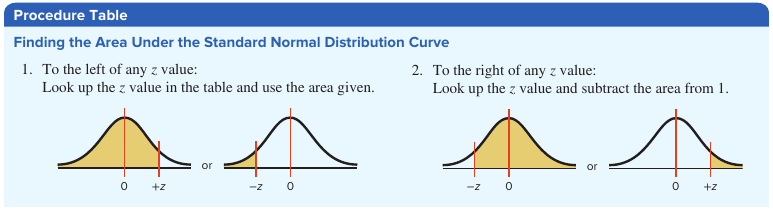
\includegraphics[width=\textwidth]{proc-table-1.png} \\
		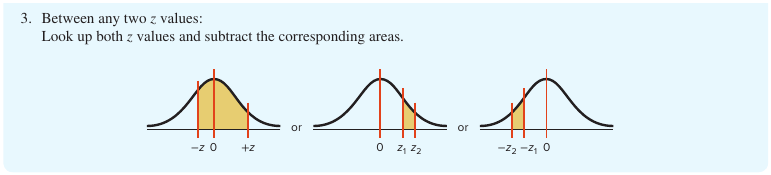
\includegraphics[width=\textwidth]{proc-table-2.png}
	\end{frame}

	\begin{frame}{Areas Under the Standard Normal Distribution}
		Find the area under the standard normal distribution curve to the left of $z = 0.50$. \pause
		
		First, draw the picture. \vspace{1.75in} \pause
		
		We're finding area to the left, so just look up the value. \pause The area is $0.6915$.
	\end{frame}

	\begin{frame}{Areas Under the Standard Normal Distribution}
		Find the area under the standard normal distribution curve to the right of $z = 1.24$. \pause
		
		First, draw the picture. \vspace{1.75in} \pause
		
		We're finding area to the right, so look up the value and subtract from $1$. \pause The area is $1 - 0.8925 = 0.1075$
	\end{frame}

	\begin{frame}{Areas Under the Standard Normal Distribution}
		Find the area under the standard normal distribution curve between $z = -1.12$ and $z = 0.94$. \pause
		
		First, draw the picture. \vspace{1.6in} \pause
		
		We're finding the area between two $z$-scores. Look up each value and subtract. \pause The area is $0.8264 - 0.1314 = 0.6950$
	\end{frame}

	\begin{frame}{Normal Curve as a Probability Density Function}
		The area under the standard normal distribution curve can also be thought of as a probability. \pause
		
		The process for solving a problem involving probability is identical to the process we just used to find the area under the curve.
	\end{frame}

	\begin{frame}{Normal Curve as a Probability Density Function}
		Find $P(0 < z < 2.53)$. \pause
		
		First, draw the picture. \vspace{1.75in} \pause
		
		Look up each value, and subtract. \pause $P(0 < z < 2.53) = 0.9943 - 0.5000 = 0.4943$
	\end{frame}

	\begin{frame}{Normal Curve as a Probability Density Function}
		Find $P(z > 1.72)$. \pause
		
		First, draw the picture. \pause \vspace{1.75in}
		
		Look up the value, then subtract from $1$. \pause $P(z > 1.72) = 1 - 0.9573 = 0.0427$
	\end{frame}

	\begin{frame}{Finding $z$-Score Given Area}
		To find a $z$-score given an area under the standard normal curve: \pause
		
		1) Draw a picture, and ``convert" it to one in which you know the area to the left of a certain $z$-score. \pause
		
		2) Find the value on the table - this is your target $z$-score. If the exact value isn't in the table, take the closest one. If it's a tie, pick the larger $z$-score.
	\end{frame}

	\begin{frame}{Finding $z$-Score Given Area}
		Find the $z$ value such that the area under the standard normal distribution curve between $0$ and the $z$ value is $0.3158$. \pause
		
		First, draw the figure and ``convert" it. \pause \vspace{1.5in}
		
		There is no $z$ score with an area of $0.8158$. A $z$ score or $0.89$ maps to $0.8133$, and a $z$ score of $0.90$ maps to $0.8159$. So we choose $z = 0.90$.
	\end{frame}

	\begin{frame}{Finding $z$-Score Given Area}
		Find the $z$ value that corresponds to the given value.
		
		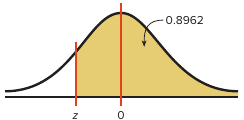
\includegraphics[width=3in]{find-z.png} \pause
		
		If the area to the \textit{right} is $0.8962$, then the area to the \textit{left} is $1 - 0.8962 = 0.1038$. \pause
		
		Consulting the table, we see that a $z$-score of $-1.26$ maps to $0.1038$.
	\end{frame}

	\begin{frame}{Next Steps}
		\begin{itemize}
			\item Complete Assignment \#8
			\item Begin Module \#10 \begin{itemize}
				\item Read 6-2
				\item Watch Video Lesson \#18
			\end{itemize}
		\end{itemize} \vfill
	
		Thanks for watching!
	\end{frame}
	
\end{document}